\documentclass[jou]{apa6}

\usepackage[american]{babel}

\usepackage{csquotes}
\usepackage[style=apa,sortcites=true,sorting=nyt,backend=biber]{biblatex}
\DeclareLanguageMapping{american}{american-apa}
\addbibresource{bibliography.bib}

\title{A Possible System Design for Large Scale Music Recommendation Applications}

\author{Nianze Liu}
\affiliation{New York University}

\leftheader{Liu}

\abstract{This article overviews a possible system design
for a large scale online music recommendation applications 
such as Spotify and Pandora, introduces a possible way for 
calculating content-based similarities based on collaborative filtering method 
in large scale, and discusses a possible music recommendation system 
based on automatical playlist generation taking use of this music similarity calculation
in the large scale.}

\keywords{Music information retrieval, Music Recommendation Systems}

\begin{document}
\maketitle

\section{Introduction}
Online music streaming applications such as Spotify and Pandora are popular
nowadays, and one of the key functions people like to use these applications 
are that they are able to recommend good music to users based on their preferences. 
Based on listeners' profile and play history, these applications are able to generate
a playlist consisting of recommended songs that the listeners might enjoy. With more 
data/history collected from listeners, the system grows more familiar with clients'
preferences, and the recommendation gets higher adoption rate, making the system more 
favorable by its users. With more and more users enjoy the streaming service, 
more and more musicians are willing to publish their new albums on the platform, 
leading to a win-win solution for both listeners and musicians, and the music
streaming platform benefits by either showing 3rd party advertisements or 
providing premium membership services.

In the light of the logic above, the key part for building a successful online music 
streaming application is to be able to generate good recommendation music playlists 
that keep clients in favor. Based on different context, there are different meanings 
for 'good'. Typically speaking, there are two kinds of recommendation systems for 
definition of goodness: user-based one and content-based one. 

User-based recommendation is also known as collaborative filter(CF) methods. 
The main idea behind this method is that if both of two listeners 
(say, \textsf{listener a} and \textsf{listener b}) like 10 music pieces, then we make the assumption that
they share the similar musical tastes, so \textsf{listener a} is likely to also enjoy 
the 11th music appearing in \textsf{listener b}'s playlist for favorate songs. 
In fact, this idea is so general that it is not restricted in music recommendation but
also applicable for other recommendations such as online shopping applications like Amazon. 
Basically, definition of 'good' in this context means 'similar users'. To generate good 
music playlist is to clustering similar listeners sharing the similar music tastes 
into the same group, and within that group the recommendation system just needs to 
push songs appearing in one user's playlist but missing in another's.

Content-based recommendation, on the other hand, differs from the collaborative filter 
methods in that its definition of 'good' is based on recommendation target's similarity.
In another word, good recommendation is given by measuring how similar the content of 
different music pieaces are. If a listener likes \textsf{music 1}, and based on similarity
calculation on music content, \textsf{music 2} is the closest song to \textsf{music 1},
then it is likely that the same listener will enjoy \textsf{music 2}. In this way, the 
recommendation playlist is generated by clustering similar musics based on their content.

In reality, according to \textcite{barrington2009smarter}, user-based 
recommendation can usually out-perform the content-based one  and has the
advantage of passive data collection: the system does not actively compute the similarity
based on music content, but just collect user's playlist and history for favorate songs 
to clustering similar users. However, there are also problems for user-based collaborative
filtering methos: first, it's hard to build all user profiles from scratch. This is 
also known as the "cold start" problem, where the system's initial state is hard to establish.
Users have to provide their initial favorate songs as seed data, and then the system is 
able to find similar users and do recommendations. Imagine how hard this will be for 
a startup company who wants to attract new customers to begin with in this situation. 
Second, even if we are able to establish the initial user profiles by some magic, 
the a problem of "cold start" continues to exist, because for any new songs released 
in the system, since nobody listens to it before, it is in nobody's playlist, 
so it is very unlikely that the new songs will be recommended
in listener's playlist. Soon or later, after listening to the same playlist for thousands 
times, the recommendation system becomes less effective.

\section{Optimizing Content-based Similarity by Collaborative Filtering}

By the nature of content-based recommendation, there's no problem of 'cold start'. As long
as the music's quality has something in common, no matter it's an old song or a new song, 
the recommendation system still works. Now, the only problem for content-based recommendation
is to raise its performance. 

In order to do so, there is a brilliant solution to optimize content-based similarity 
by the help of collaborative filtering method. According to \textcite{mcfee2010learning},
the key is to group similar artists by the help of collaborative filtering data, forming 
similar artist groups, and then calculate the music content-based similarity based on these
groups.

Specifically, to find similar artist, a collaborative filtering matrix \textsf{F} is constructed
based on the online open data from Last.fm and Swat10k, where
each column represents an artist, and each row stands for different users. If a user \textsf{u} 
listens to songs from artist \textsf{i}, then \textsf{Fui} will be marked as 1, otherwise it is 0. Each artist is thus represented by a column vector, and by calculating the 
cosine-similarity between two different columns, we can get the distance for corresponding two artist. 
For each artist, the relavent artists group is generated by selecting 10 closest artists 
according to this distance.

After we get the relavent artists groups, each of which has a size of 11, within the group, 
we combine their music pieces into the same union set, and calculate the content-based similarity
inside this union set. In such a way, the content-based recommendation is firstly filtered by 
collaborative filtering method, which act as the first optimization. In order to further 
refine the music content distance, according to \textcite{mcfee2010metric}, more advanced 
techniques such as Metric Learning to Rank could be adopted to furture optimize the result.

\section{Typical Information Retrieval System in Large Scale}

As talked above, the key part of music recommendation system is to build a highly 
effective system to handle query-by-example paradigm, so that given a random music piece, 
we can return a list of similar music pieces and they are ordered in a playlist in a nice way. 
By combining optimized content-based similarity mentioned above with a typical information
 retrieval system, it is possible to build such a recommendation system in large scale.

A typicall information retrieval system backed by machine-learned engine, according to wikipedia, is shown in 
Figure~\ref{fig:Figure1}, which consists of two phases. Basically, we want to retrieve the 
results as soon as possible, so given the query, we firstly get a group of candidates from 
database with fast retrieval algorithms such as weighted AND according to 
\textcite{broder2003efficient} in the first phase with larger granularity but less 
computational requirement, and then we reorder these candidates by machine-learned 
models before sending back the final result in the second more computational heavy phase.

\begin{figure}[h!]
  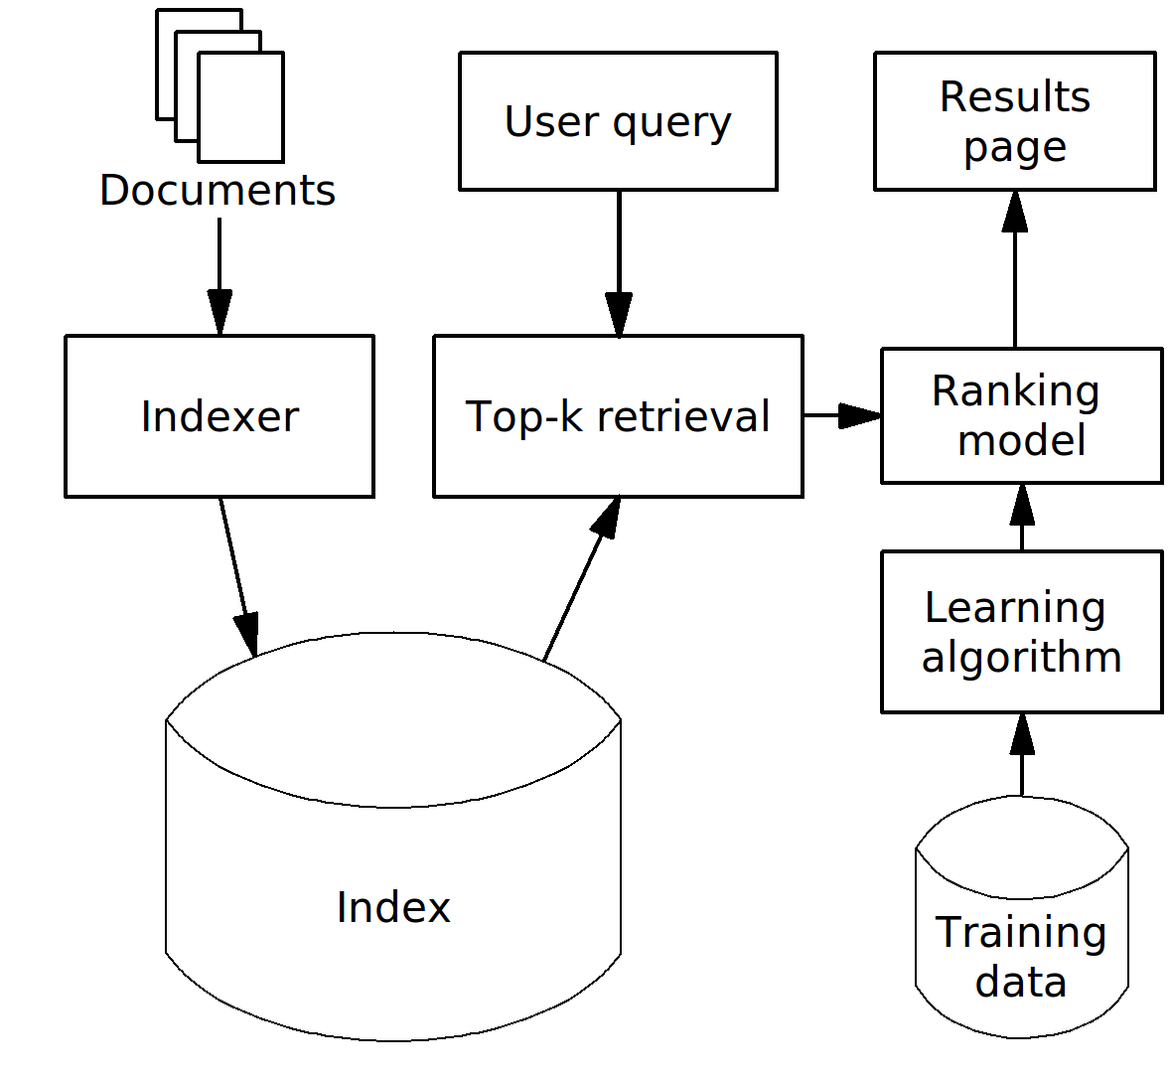
\includegraphics[width=\linewidth]{MLR-search-engine-example.png}
  \caption{A Typical Information Retrieval System.}
  \label{fig:Figure1}
\end{figure}

\section{A Possible Music Recommendation System in Large Scale}

The optimized content-based similarity by collaborative filtering could be adapted into the typical information retrieval system mentioned above. The top-k retrieval in the typical
large scale system might be replaced by returning the union set of music pieces built by 
relavent artists using CF matrix. Another possible way to achieve this quick candidate 
retrieval, according to \textcite{mcfee2011large}, is using spatial trees to get top-k 
result. Then in the second phase, by computing the content-based similarity and using Metric Learning to Rank algorithms mentioned in \textcite{mcfee2010metric}, an ordered playlist is generated. By using this generated ordered list to millions of users in large scale, it is possible to 
build an online music recommendation application now.

\printbibliography

\end{document}